\documentclass{standalone}

\usepackage{tikz}
    \usetikzlibrary{arrows.meta}
    \usetikzlibrary{calc}
    \usetikzlibrary{decorations.pathmorphing}

\tikzset{
    bluearrow/.style={
        blue!25,
        -{Kite[length=2.5mm]}, 
        line width=0.5mm,},
    greensq/.style={
        green,
        fill=green!20, 
        line width=0.4mm,},
    redsq/.style={
        red,
        fill=red!20, 
        line width=0.4mm,},
    }
    
\begin{document}
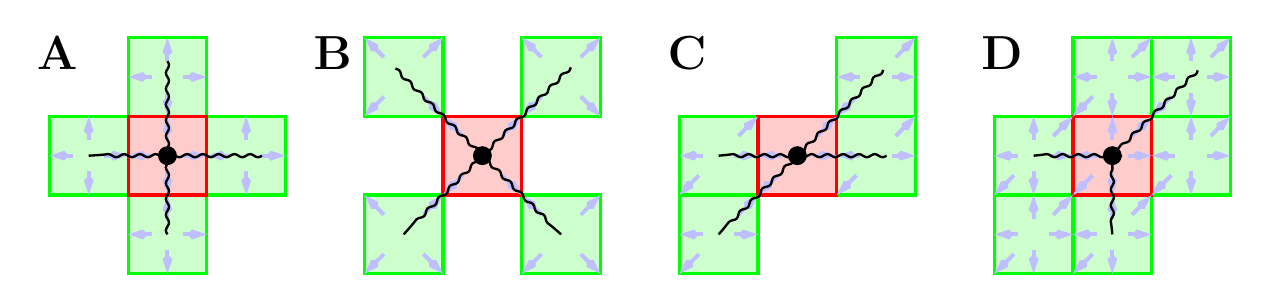
\begin{tikzpicture}
    % \draw[help lines] (0,0) grid (15,3);
    \foreach \x in % green
        {(1,0), (0,1), (2,1), (1,2),% case (A)
         (4,0), (6,0), (4,2), (6,2), % case (B)
         (8,0), (8,1), (10,1), (10,2),% case (C)
         (13,0), (13,2), (12,1), (14,1), (12,0), (14,2)% case (D6)
        } 
        {\draw[greensq] \x rectangle+(1,1);} 
    \foreach \x in % red
        {(1,1), (5,1), (9,1), (13,1)} 
        {\draw[redsq] \x rectangle+(1,1);}
   
    \fill[black] 
        (1.5,1.5) circle (1.2mm)
        (5.5,1.5) circle (1.2mm)
        (9.5,1.5) circle (1.2mm)
        (13.5,1.5) circle (1.2mm);
    % case (A) bound
    \foreach \x in
        {(1,0), (0,1), (2,1), (1,2), (1,1)} 
        {\draw[bluearrow] \x++(0.3,0.5) -- ++(-0.3,0);
         \draw[bluearrow] \x++(0.7,0.5) -- ++(0.3,0);
         \draw[bluearrow] \x++(0.5,0.3) -- ++(0,-0.3);
         \draw[bluearrow] \x++(0.5,0.7) -- ++(0,0.3);}
    % case (B) bound
    \foreach \x in
        {(4,0), (6,0), (4,2), (6,2), (5,1)} 
        {\draw[bluearrow] \x++(0.25,0.75) -- ++(-.25,0.25);
         \draw[bluearrow] \x++(0.25,0.25) -- ++(-0.25,-0.25);
         \draw[bluearrow] \x++(0.75,0.75) -- ++(.25,0.25);
         \draw[bluearrow] \x++(0.75,0.25) -- ++(0.25,-0.25);}
    % case (C) bound
    \foreach \x in
        {(8,0), (8,1), (10,1), (10,2), (9,1)} 
        {\draw[bluearrow] \x++(0.25,0.25) -- ++(-0.25,-0.25);
         \draw[bluearrow] \x++(0.75,0.75) -- ++(.25,0.25);
         \draw[bluearrow] \x++(0.3,0.5) -- ++(-0.3,0);
         \draw[bluearrow] \x++(0.7,0.5) -- ++(0.3,0);}
    % case (D6) bound
    \foreach \x in
        {(13,0), (13,2), (12,1), (14,1), (12,0), (14,2), (13,1)} 
        {\draw[bluearrow] \x++(0.25,0.25) -- ++(-0.25,-0.25);
         \draw[bluearrow] \x++(0.75,0.75) -- ++(.25,0.25);
         \draw[bluearrow] \x++(0.3,0.5) -- ++(-0.3,0);
         \draw[bluearrow] \x++(0.7,0.5) -- ++(0.3,0);
         \draw[bluearrow] \x++(0.5,0.3) -- ++(0,-0.3);
         \draw[bluearrow] \x++(0.5,0.7) -- ++(0,0.3);}
    \draw[line width=0.3mm, decorate, decoration={coil,aspect=0,segment length=2mm,amplitude=0.2mm}]
        (1.5,0.5)--(1.5,2.5) 
        (0.5,1.5)--(2.5,1.5)
        (4.5,0.5)--(6.5,2.5) 
        (6.5,0.5)--(4.5,2.5)
        (8.5,0.5)--(10.5,2.5) 
        (8.5,1.5)--(10.5,1.5)
        (13.5,1.5)--(14.5,2.5) 
        (12.5,1.5)--(13.5,1.5) 
        (13.5,0.5)--(13.5,1.5);
    \node at (0.1,2.8){\LARGE{\bf A}};
    \node at (3.6,2.8){\LARGE{\bf B}};
    \node at (8.1,2.8){\LARGE{\bf C}};
    \node at (12.1,2.8){\LARGE{\bf D}};
\end{tikzpicture}
\end{document}